\chapter{Participant data}

These are the results of the measurements from Experiment one for each participant. 

\subsection{Graph descriptions}

\subsubsection{Accelerometer}
The accelerometer graph shows the changes of the three axis values over the time of the experiment. 

\subsubsection{Noise and Light}
The graphs of the noise and light level show the changes of the measurements (y-axis) over time (x-axis). 
The the thicker horizontal line indicates the average value and two lines, one below and the other one on top of the average is the range of the standard deviation and is treated different in the evaluation section.

\clearpage
\section{Participant 1}

\subsection{date \& time}
\begin{table}[ht]
  \begin{tabular}{|P{3cm}|P{3cm}|}
	\multicolumn{2}{c}{\textbf{2016-08-03}}    	\\ \hline
    Start Time      			& End Time   					\\ \hline
   \textbf{15:38:54} 	& \textbf{15:56:12}    	\\ \hline
   \multicolumn{2}{c}{Duration}    						\\ \hline
   \multicolumn{2}{c}{\textbf{00:17:18}} 			\\ \hline
  \end{tabular}
  \newline\newline
  \caption{p1: date and time}\label{dandt1}
\end{table}

\subsection{Questions}
\begin{itemize}
  \item[\Checkmark] Are you a Student?
  \item[\XSolidBrush] Did you work in a team?
  \item[\XSolidBrush] Did you listen to music?
  \item[\Checkmark] Did you feel tired?
  \item[\XSolidBrush] Did you enjoy the tasks?
  \item[\XSolidBrush] Did you give all you attention to the tasks?
  \item[\XSolidBrush] Were you distracted during the tasks?
  \item[\Checkmark] Did you feel stressed
  \item[\XSolidBrush] Do you think the tasks were easy?  
\end{itemize}

\newpage

\subsection{Accelerometer}
\begin{figure}[ht]
	\centering
	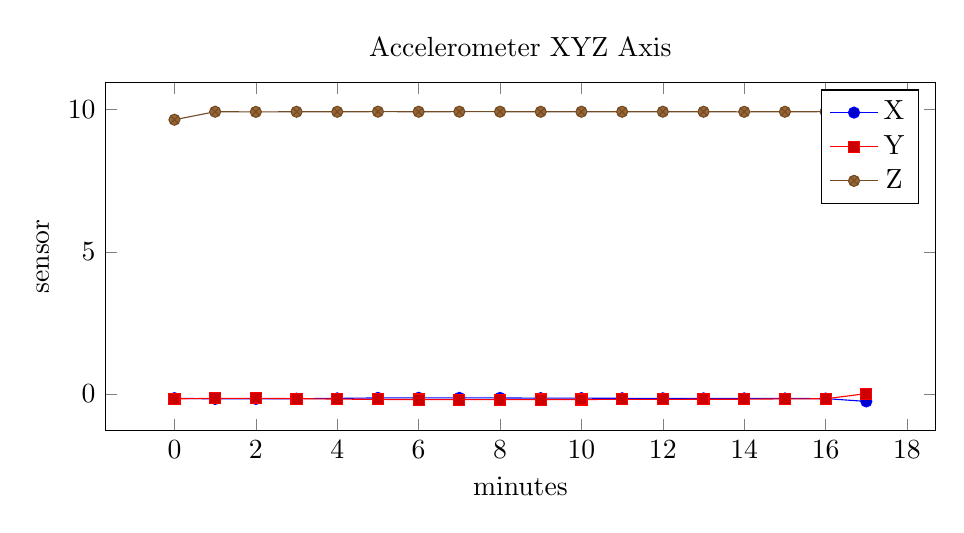
\begin{tikzpicture}
\begin{axis}[
	height=6cm,
	width=\textwidth,
	xlabel=minutes,
	ylabel=sensor,
	title=Accelerometer XYZ Axis,
	unbounded coords=discard],
	
%X
\addplot coordinates {
(0 , -0.144712392571)
(1 , -0.171607927941)
(2 , -0.170622079706)
(3 , -0.162515509394)
(4 , -0.151926182059)
(5 , -0.135589277353)
(6 , -0.132913407353)
(7 , -0.134673849412)
(8 , -0.135671431818)
(9 , -0.144321071176)
(10 , -0.143968983235)
(11 , -0.149250311471)
(12 , -0.150024906176)
(13 , -0.152322015758)
(14 , -0.152559941765)
(15 , -0.156679375)
(16 , -0.158615859706)
(17 , -0.258813207)
};

%Y
\addplot coordinates {
(0 , -0.17022774)
(1 , -0.149285518824)
(2 , -0.151151587353)
(3 , -0.160048757273)
(4 , -0.176325913529)
(5 , -0.187980040294)
(6 , -0.193965545882)
(7 , -0.195585153235)
(8 , -0.195780402121)
(9 , -0.193296577941)
(10 , -0.191571342647)
(11 , -0.185761882941)
(12 , -0.185902718235)
(13 , -0.183047602727)
(14 , -0.180586184118)
(15 , -0.168051834118)
(16 , -0.165798468824)
(17 , 0.01532289)
};

%Z
\addplot coordinates {
(0 , 9.64186077143)
(1 , 9.9233675)
(2 , 9.91780444118)
(3 , 9.92204354545)
(4 , 9.92065644118)
(5 , 9.92477579412)
(6 , 9.92287461765)
(7 , 9.92414205882)
(8 , 9.92422)
(9 , 9.92181826471)
(10 , 9.92354352941)
(11 , 9.92209991176)
(12 , 9.92389579412)
(13 , 9.92153551515)
(14 , 9.91977617647)
(15 , 9.92181838235)
(16 , 9.92442373529)
(17 , 9.9312684)
};

\addlegendentry{X}
\addlegendentry{Y}
\addlegendentry{Z}
\end{axis}
\end{tikzpicture}
	\vspace{5 mm}
\end{figure}

\FloatBarrier

\subsection{Light}
\begin{figure}[ht]
	\centering
	\begin{tikzpicture}
\begin{axis}[
	height=6cm,
	width=\textwidth,
	xlabel=minutes,
	ylabel=sensor,
	title=Light,
	unbounded coords=discard],
	
\addplot coordinates {
(0 , 0.0)
(1 , 0.0)
(2 , 0.0)
(3 , 0.0)
(4 , 0.0)
(5 , 0.0)
(6 , 0.0)
(7 , 0.0)
(8 , 0.0)
(9 , 0.0)
(10 , 0.0)
(11 , 0.0)
(12 , 0.0)
(13 , 0.0)
(14 , 0.0)
(15 , 0.0)
(16 , 0.0)
(17 , 0.0)
};

\end{axis}
\end{tikzpicture}
	\vspace{5 mm}
\end{figure}

\newpage
\FloatBarrier

\subsection{Volume}
\begin{figure}[ht]
	\centering
	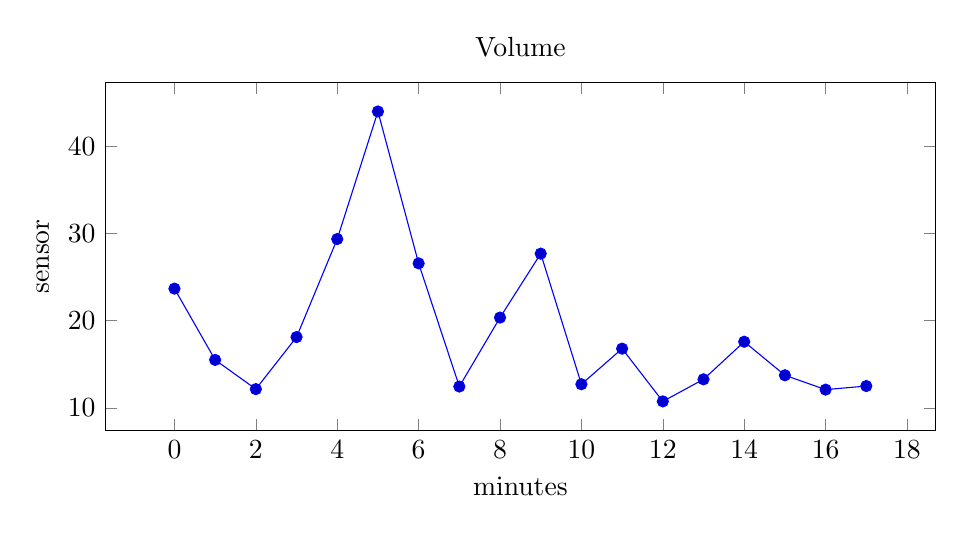
\begin{tikzpicture}
\begin{axis}[
	height=6cm,
	width=\textwidth,
	xlabel=minutes,
	ylabel=sensor,
	title=Volume,
	unbounded coords=discard],

\addplot coordinates {
(0 , 23.6857142857)
(1 , 15.5)
(2 , 12.1470588235)
(3 , 18.1212121212)
(4 , 29.3823529412)
(5 , 44.0294117647)
(6 , 26.5882352941)
(7 , 12.4411764706)
(8 , 20.3636363636)
(9 , 27.7058823529)
(10 , 12.7058823529)
(11 , 16.7941176471)
(12 , 10.7352941176)
(13 , 13.2727272727)
(14 , 17.5882352941)
(15 , 13.7352941176)
(16 , 12.0882352941)
(17 , 12.5)
};

\end{axis}
\end{tikzpicture}
 	\vspace{5 mm}
\end{figure}

\FloatBarrier

\subsection{Location}
No data gathered
\clearpage
\section{Participant 2}

% JC

\subsection{Date \& Time}
\begin{table}[ht]
  \begin{tabular}{|P{3cm}|P{3cm}|}
	\multicolumn{2}{c}{\textbf{2016-08-03}}    	\\ \hline
    Start Time      			& End Time   					\\ \hline
   \textbf{12:23:50} 	& \textbf{12:42:23}    	\\ \hline
   \multicolumn{2}{c}{Duration}    						\\ \hline
   \multicolumn{2}{c}{\textbf{00:18:33}} 			\\ \hline
  \end{tabular}
  \newline\newline
  \caption{P2: Date and Time}\label{dandt2}
\end{table}

\subsection{Questions}
\begin{itemize} 
  \item[\XSolidBrush] Are you a Student?
  \item[\Checkmark] Did you work in a team?
  \item[\Checkmark] Did you listen to music?
  \item[\XSolidBrush] Did you feel tired?
  \item[\Checkmark] Did you enjoy the tasks?
  \item[\Checkmark] Did you give all you attention to the tasks?
  \item[\XSolidBrush] Were you distracted during the tasks?
  \item[\XSolidBrush] Did you feel stressed
  \item[\Checkmark] Do you think the tasks were easy?  
\end{itemize}


\FloatBarrier
\newpage
\subsection{Accelerometer}

\begin{figure}[ht]
	\centering
	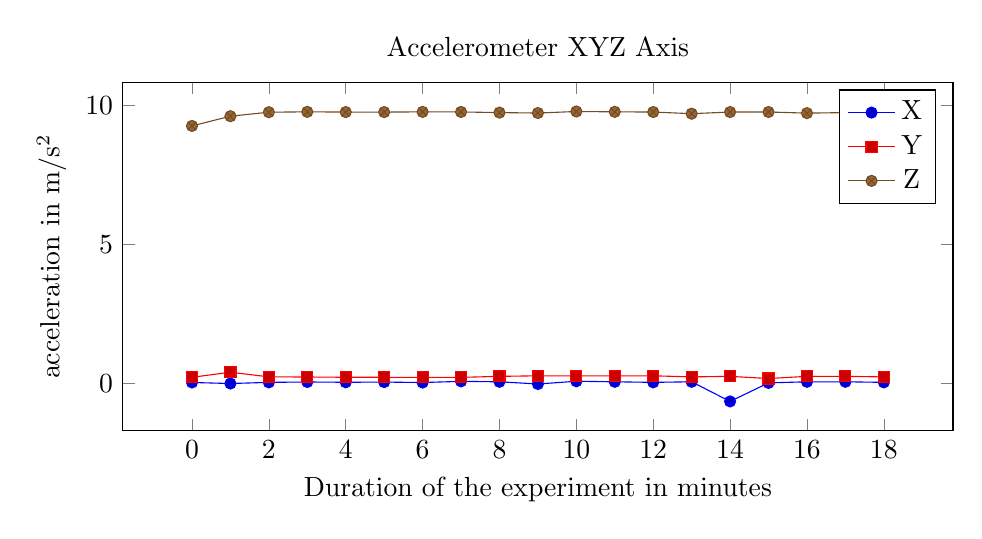
\begin{tikzpicture}
\begin{axis}[
	height=6cm,
	width=\textwidth,
	xlabel=Duration of the experiment in minutes,
	ylabel=acceleration in m/s$^2$,
	title=Accelerometer XYZ Axis,
	unbounded coords=discard],
	
%X
\addplot coordinates {
(0 , 0.0349651822609)
(1 , -0.00309673126316)
(2 , 0.0382930208571)
(3 , 0.0523034957619)
(4 , 0.0420292439048)
(5 , 0.049033425)
(6 , 0.0326879590952)
(7 , 0.0751864109167)
(8 , 0.05883789)
(9 , -0.019607544)
(10 , 0.07846069)
(11 , 0.05883789)
(12 , 0.039230347)
(13 , 0.05883789)
(14 , -0.64723206)
(15 , 0.019607544)
(16 , 0.05883789)
(17 , 0.05883789)
(18 , 0.039230347)
};

%Y
\addplot coordinates {
(0 , 0.220863674783)
(1 , 0.403620667895)
(2 , 0.23722984381)
(3 , 0.231626238095)
(4 , 0.222285678571)
(5 , 0.221095690909)
(6 , 0.217615762857)
(7 , 0.219015755833)
(8 , 0.25497437)
(9 , 0.2745819)
(10 , 0.2745819)
(11 , 0.2745819)
(12 , 0.2745819)
(13 , 0.23536682)
(14 , 0.25497437)
(15 , 0.17651367)
(16 , 0.25497437)
(17 , 0.25497437)
(18 , 0.23536682)
};

%Z
\addplot coordinates {
(0 , 9.26770895652)
(1 , 9.61774347368)
(2 , 9.76181833333)
(3 , 9.77489447619)
(4 , 9.76648904762)
(5 , 9.76563831818)
(6 , 9.77396304762)
(7 , 9.77069233333)
(8 , 9.74780316161)
(9 , 9.73178425312)
(10 , 9.78743477033)
(11 , 9.77489304762)
(12 , 9.76742633556)
(13 , 9.70858834222)
(14 , 9.76742655645)
(15 , 9.76935722354)
(16 , 9.72819595862)
(17 , 9.74780318532)
(18 , 9.70858858813)
};

\addlegendentry{X}
\addlegendentry{Y}
\addlegendentry{Z}
\end{axis}
\end{tikzpicture}
 	\vspace{5 mm}
\end{figure}

\FloatBarrier
\subsection{Light Level}
\begin{figure}[ht]
	\centering
	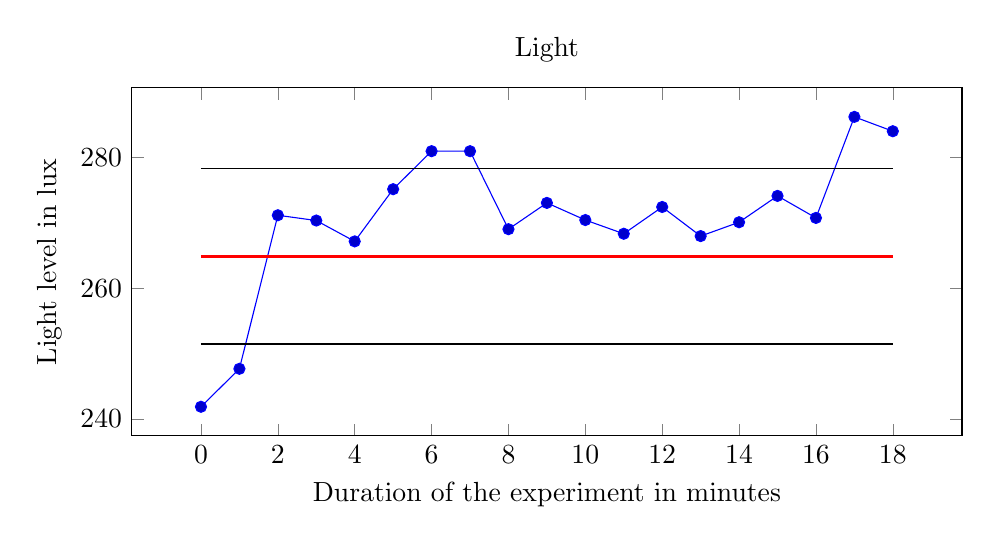
\begin{tikzpicture}
\begin{axis}[
	height=6cm,
	width=\textwidth,
	xlabel=Duration of the experiment in minutes,
	ylabel=Light level in lux,
	title=Light,
	unbounded coords=discard],
	
\addplot coordinates {
(0 , 241.869565217)
(1 , 247.684210526)
(2 , 271.19047619)
(3 , 270.380952381)
(4 , 267.19047619)
(5 , 275.181818182)
(6 , 281.0)
(7 , 281.0)
(8 , 269.056565454)
(9 , 273.082245)
(10 , 270.457685359)
(11 , 268.358045125)
(12 , 272.456782138)
(13 , 268.0)
(14 , 270.121246868)
(15 , 274.154865478)
(16 , 270.782398425)
(17 , 286.252546845)
(18 , 284.054086785)
};

\addplot[mark=none, red, very thick] coordinates {(0, 264.928214098) (18, 264.928214098)};

\addplot[mark=none, black] coordinates {(0, 251.47691699) (18, 251.47691699)};
\addplot[mark=none, black] coordinates {(0, 278.379511206) (18, 278.379511206)};

\end{axis}
\end{tikzpicture}
 	\vspace{5 mm}
\end{figure}

\newpage
\FloatBarrier
\newpage
\subsection{Noise Level}
\begin{figure}[ht]
	\centering
	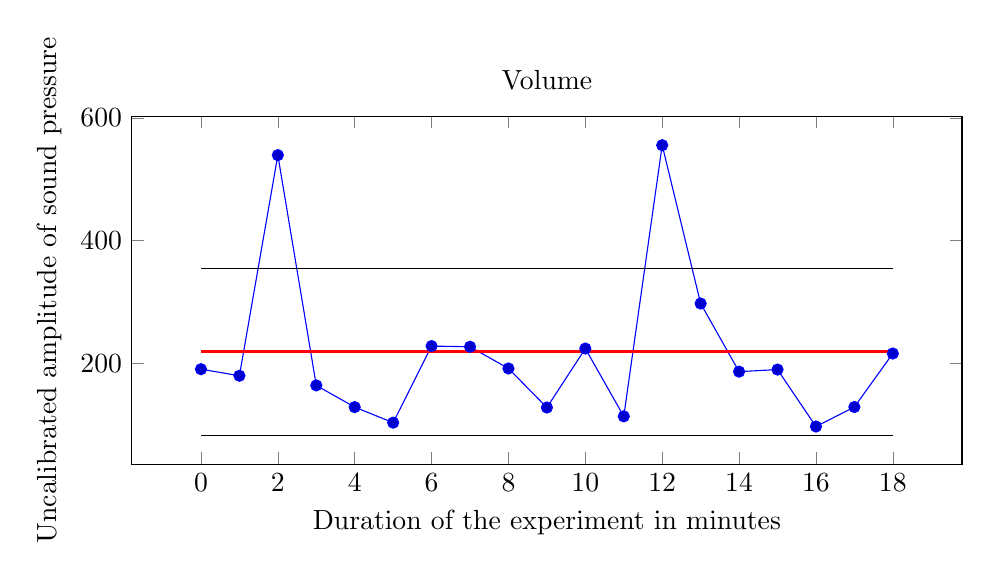
\begin{tikzpicture}
\begin{axis}[
	height=6cm,
	width=\textwidth,
	ylabel=Uncalibrated amplitude of sound pressure,
	xlabel=Duration of the experiment in minutes,
	title=Volume,
	unbounded coords=discard],

\addplot coordinates {
(0 , 190.434782609)
(1 , 179.736842105)
(2 , 539.238095238)
(3 , 164.0)
(4 , 128.619047619)
(5 , 103.318181818)
(6 , 228.095238095)
(7 , 227.0)
(8 , 191.596186522)
(9 , 127.958334583)
(10 , 224.056548712)
(11 , 113.580190875)
(12 , 555.4568753253)
(13 , 297.4565454254)
(14 , 186.4298341674)
(15 , 189.8012096456)
(16 , 97.0)
(17 , 128.8121400108)
(18 , 215.9958225684)
};

\addplot[mark=none, red, very thick] coordinates {(0, 219.063169641) (18, 219.063169641)};

\addplot[mark=none, black] coordinates {(0, 83.0123913636) (18, 83.0123913636)};
\addplot[mark=none, black] coordinates {(0, 355.113947918) (18, 355.113947918)};

\end{axis}
\end{tikzpicture}
 	\vspace{5 mm}
\end{figure}

\FloatBarrier

\subsection{Location}
minute 0 : -3.6881917, 40.4579957
minute 1 : -3.68815341053, 40.4579801474)
from minute 2 : -3.6881432, 40.457976)

Madrid, Spain 

\FloatBarrier
\clearpage
\section{Participant 3}

\subsection{date \& time}
\begin{table}[ht]
  \begin{tabular}{|P{3cm}|P{3cm}|}
	\multicolumn{2}{c}{\textbf{2016-07-28}}    	\\ \hline
    Start Time      			& End Time   					\\ \hline
   \textbf{12:52:44} 	& \textbf{13:04:45}    	\\ \hline
   \multicolumn{2}{c}{Duration}    						\\ \hline
   \multicolumn{2}{c}{\textbf{00:12:01}} 			\\ \hline
  \end{tabular}
  \newline\newline
 \caption{p3: date and time}\label{dandt1}
\end{table}

\subsection{Questions}
\begin{itemize} 
  \item[\Checkmark] Are you a Student?
  \item[\XSolidBrush] Did you work in a team?
  \item[\Checkmark] Did you listen to music?
  \item[\XSolidBrush] Did you feel tired?
  \item[\Checkmark] Did you enjoy the tasks?
  \item[\Checkmark] Did you give all you attention to the tasks?
  \item[\XSolidBrush] Were you distracted during the tasks?
  \item[\XSolidBrush] Did you feel stressed
  \item[\XSolidBrush] Do you think the tasks were easy?  
\end{itemize}


\FloatBarrier
\newpage
\subsection{Accelerometer}

\begin{figure}[ht]
	\centering
	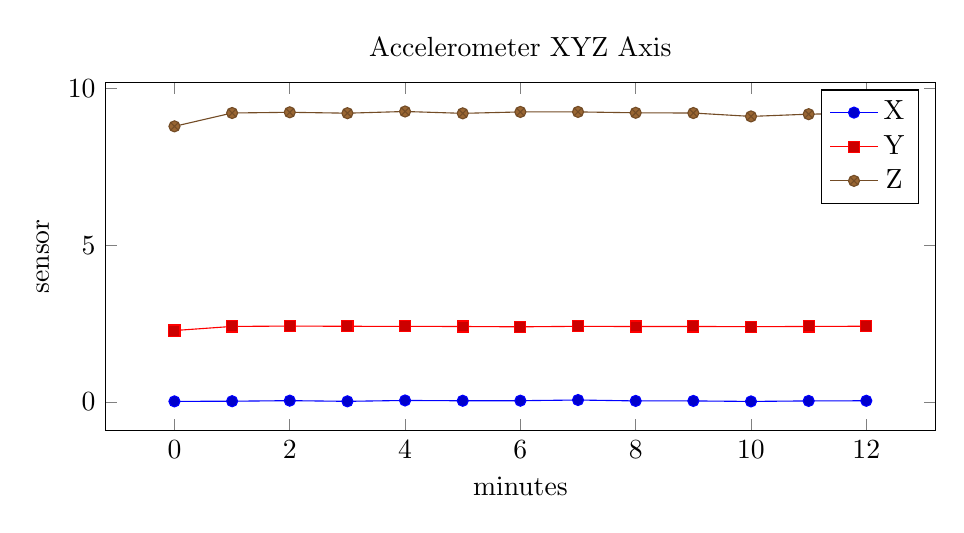
\begin{tikzpicture}
\begin{axis}[
	height=6cm,
	width=\textwidth,
	xlabel=minutes,
	ylabel=sensor,
	title=Accelerometer XYZ Axis,
	unbounded coords=discard],
	
%X
\addplot coordinates {
(0 , 0.019438637881)
(1 , 0.0247400849444)
(2 , 0.0424115735714)
(3 , 0.02101577)
(4 , 0.0486535994286)
(5 , 0.0389057787143)
(6 , 0.041366485)
(7 , 0.0629475533333)
(8 , 0.034117374125)
(9 , 0.033618582)
(10 , 0.0179565136667)
(11 , 0.0341173747143)
(12 , 0.038905777)
};

%Y
\addplot coordinates {
(0 , 2.2777979)
(1 , 2.40836742222)
(2 , 2.42019587143)
(3 , 2.41288974444)
(4 , 2.41164518571)
(5 , 2.40600168571)
(6 , 2.39666241111)
(7 , 2.4114599)
(8 , 2.4058734375)
(9 , 2.40826766667)
(10 , 2.3990899)
(11 , 2.40848141429)
(12 , 2.4145525)
};

%Z
\addplot coordinates {
(0 , 8.7865777619)
(1 , 9.21202333333)
(2 , 9.234265)
(3 , 9.20590511111)
(4 , 9.26008828571)
(5 , 9.20108792857)
(6 , 9.24580855556)
(7 , 9.24680616667)
(8 , 9.2185745)
(9 , 9.21099291667)
(10 , 9.1032535)
(11 , 9.17449528571)
(12 , 9.20391)
};

\addlegendentry{X}
\addlegendentry{Y}
\addlegendentry{Z}
\end{axis}
\end{tikzpicture}
 	\vspace{5 mm}
\end{figure}

\FloatBarrier
\subsection{Light}
\begin{figure}[ht]
	\centering
	\begin{tikzpicture}
\begin{axis}[
	height=6cm,
	width=\textwidth,
	xlabel=minutes,
	ylabel=sensor,
	title=Light,
	unbounded coords=discard],
	
\addplot coordinates {
(0 , 330.986057143)
(1 , 327.141866667)
(2 , 324.539771429)
(3 , 322.701066667)
(4 , 329.208342857)
(5 , 335.669942857)
(6 , 346.047466667)
(7 , 352.541066667)
(8 , 368.9453)
(9 , 374.263066667)
(10 , 355.196133333)
(11 , 340.515885714)
(12 , 332.4064)
};

\end{axis}
\end{tikzpicture}
 	\vspace{5 mm}
\end{figure}

\newpage
\FloatBarrier
\newpage
\subsection{Volume}
\begin{figure}[ht]
	\centering
	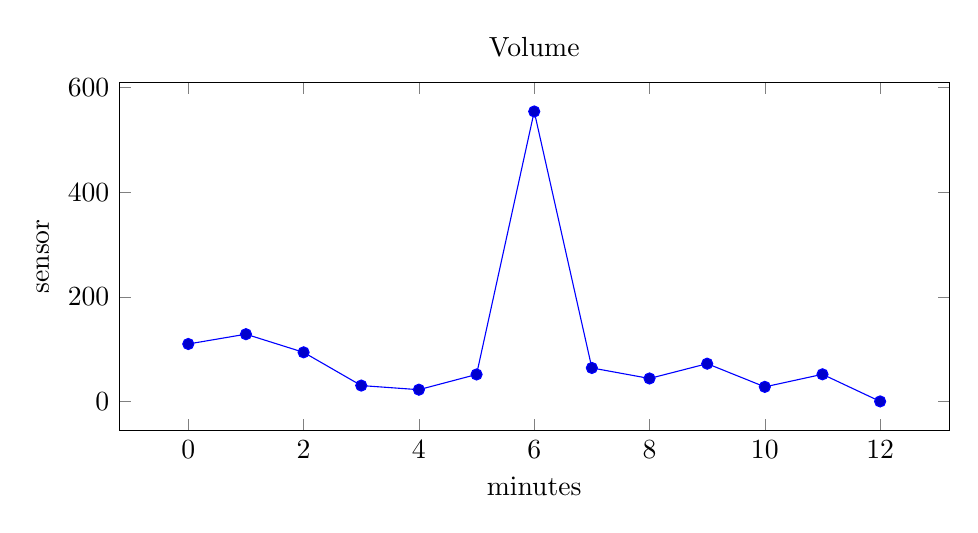
\begin{tikzpicture}
\begin{axis}[
	height=6cm,
	width=\textwidth,
	xlabel=minutes,
	ylabel=sensor,
	title=Volume,
	unbounded coords=discard],

\addplot coordinates {
(0 , 109.80952381)
(1 , 128.555555556)
(2 , 93.8571428571)
(3 , 30.3333333333)
(4 , 22.4285714286)
(5 , 51.5714285714)
(6 , 554.333333333)
(7 , 64.0)
(8 , 43.875)
(9 , 72.1666666667)
(10 , 27.8333333333)
(11 , 51.8571428571)
(12 , 0.0)
};

\end{axis}
\end{tikzpicture}
 	\vspace{5 mm}
\end{figure}

\FloatBarrier
\subsection{Steps}
\begin{figure}[ht]
	\centering
	\begin{tikzpicture}
\begin{axis}[
	height=6cm,
	width=\textwidth,
	xlabel=minutes,
	ylabel=sensor,
	title=Steps,
	unbounded coords=discard],

\addplot coordinates {
(0 , 0.0)
(1 , 0.0)
(2 , 0.0)
(3 , 0.0)
(4 , 0.0)
(5 , 0.0)
(6 , 0.0)
(7 , 0.0)
(8 , 0.0)
(9 , 0.0)
(10 , 0.0)
(11 , 0.0)
(12 , 0.0)
};

\end{axis}
\end{tikzpicture}
 	\vspace{5 mm}
\end{figure}

\newpage
\FloatBarrier

\subsection{Location}
No data gathered

\FloatBarrier
\subsection{Weather}
No data gathered

\FloatBarrier
\clearpage
\section{Participant 4}

%% MK

\subsection{Date \& Time}
\begin{table}[ht]
  \begin{tabular}{|P{3cm}|P{3cm}|}
	\multicolumn{2}{c}{\textbf{2016-08-04}}    	\\ \hline
    Start Time      			& End Time   					\\ \hline
   \textbf{10:20:13} 	& \textbf{11:20:41}    	\\ \hline
   \multicolumn{2}{c}{Duration}    						\\ \hline
   \multicolumn{2}{c}{\textbf{01:00:28}} 			\\ \hline
  \end{tabular}
  \newline\newline
  \caption{P4: Date and Time}\label{dandt4}
\end{table}

\subsection{Questions}
\begin{itemize} 
  \item[\Checkmark] Are you a Student?
  \item[\XSolidBrush] Did you work in a team?
  \item[\XSolidBrush] Did you listen to music?
  \item[\Checkmark] Did you feel tired?
  \item[\Checkmark] Did you enjoy the tasks?
  \item[\XSolidBrush] Did you give all you attention to the tasks?
  \item[\Checkmark] Were you distracted during the tasks?
  \item[\Checkmark] Did you feel stressed
  \item[\XSolidBrush] Do you think the tasks were easy?  
\end{itemize}


\FloatBarrier
\newpage

\subsection{Accelerometer}

\begin{figure}[ht]
	\centering
	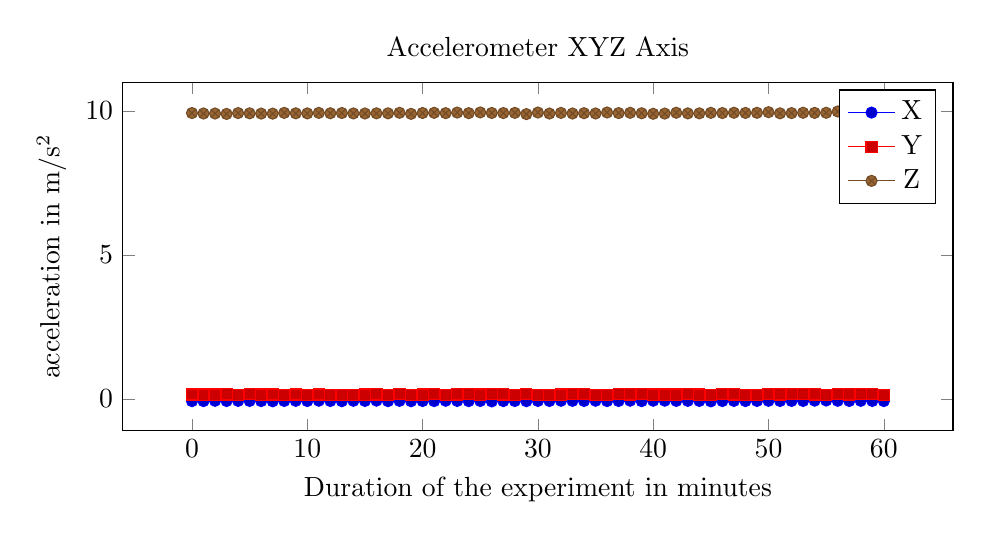
\begin{tikzpicture}
\begin{axis}[
	height=6cm,
	width=\textwidth,
	xlabel=Duration of the experiment in minutes,
	ylabel=acceleration in m/s$^2$,
	title=Accelerometer XYZ Axis,
	unbounded coords=discard],
	
%X
\addplot coordinates {
(0 , -0.0747131762353)
(1 , -0.073247608625)
(2 , -0.063521163625)
(3 , -0.070778586)
(4 , -0.06584054825)
(5 , -0.0672371646667)
(6 , -0.0736217)
(7 , -0.0798067233333)
(8 , -0.0686337833333)
(9 , -0.06434417)
(10 , -0.07122749975)
(11 , -0.0600545593333)
(12 , -0.069282211)
(13 , -0.07631518)
(14 , -0.06299743325)
(15 , -0.0679354745)
(16 , -0.0568622886667)
(17 , -0.07481880275)
(18 , -0.064643445)
(19 , -0.0770134866667)
(20 , -0.0708284676667)
(21 , -0.0723048914)
(22 , -0.061451177)
(23 , -0.0666386146667)
(24 , -0.0737214611667)
(25 , -0.06823475)
(26 , -0.0831985105)
(27 , -0.073621705)
(28 , -0.0700303985)
(29 , -0.07571663)
(30 , -0.06808510825)
(31 , -0.0690328133333)
(32 , -0.06269815775)
(33 , -0.064942722)
(34 , -0.06853402325)
(35 , -0.061052144)
(36 , -0.0724246025)
(37 , -0.0694318475)
(38 , -0.05865794)
(39 , -0.074699092)
(40 , -0.060752869)
(41 , -0.0587576993333)
(42 , -0.066638614)
(43 , -0.065241995)
(44 , -0.0673369215)
(45 , -0.082001406)
(46 , -0.071526772)
(47 , -0.06688800775)
(48 , -0.072723875)
(49 , -0.067636197)
(50 , -0.06314707)
(51 , -0.06958148675)
(52 , -0.0672371633333)
(53 , -0.068035233)
(54 , -0.0580593925)
(55 , -0.0528434535714)
(56 , -0.06254852)
(57 , -0.0688017963684)
(58 , -0.06464344625)
(59 , -0.068234749)
(60 , -0.0725243588333)
};

%Y
\addplot coordinates {
(0 , 0.156256870588)
(1 , 0.15315409)
(2 , 0.15367782375)
(3 , 0.15786767)
(4 , 0.14454993)
(5 , 0.16360378)
(6 , 0.15382746)
(7 , 0.155822623333)
(8 , 0.145846786667)
(9 , 0.155323835)
(10 , 0.15083471)
(11 , 0.155822626667)
(12 , 0.1484405075)
(13 , 0.142455)
(14 , 0.144250655)
(15 , 0.15412673)
(16 , 0.157219246667)
(17 , 0.1415571775)
(18 , 0.160411515)
(19 , 0.147442923333)
(20 , 0.154226496667)
(21 , 0.159214414)
(22 , 0.148240986667)
(23 , 0.157219246667)
(24 , 0.161508855)
(25 , 0.154126735)
(26 , 0.165499195)
(27 , 0.15682021)
(28 , 0.15203181)
(29 , 0.187047005)
(30 , 0.143352825)
(31 , 0.15003664)
(32 , 0.1550245625)
(33 , 0.16011224)
(34 , 0.1593640525)
(35 , 0.15023616)
(36 , 0.14514848)
(37 , 0.16071079)
(38 , 0.15741876)
(39 , 0.162207164)
(40 , 0.15502456)
(41 , 0.15522408)
(42 , 0.153627943333)
(43 , 0.17238252)
(44 , 0.153528185)
(45 , 0.14584679)
(46 , 0.16190789)
(47 , 0.15816695)
(48 , 0.15263036)
(49 , 0.14754268)
(50 , 0.16011224)
(51 , 0.157269125)
(52 , 0.159812963333)
(53 , 0.165997983333)
(54 , 0.15831659)
(55 , 0.147499927143)
(56 , 0.172981075)
(57 , 0.157733788421)
(58 , 0.1634042675)
(59 , 0.1726818)
(60 , 0.140360076667)
};

%Z
\addplot coordinates {
(0 , 9.92474058824)
(1 , 9.9079546875)
(2 , 9.9084784375)
(3 , 9.89433775)
(4 , 9.923517)
(5 , 9.914589)
(6 , 9.905411)
(7 , 9.90421416667)
(8 , 9.93035066667)
(9 , 9.914988)
(10 , 9.91244375)
(11 , 9.930351)
(12 , 9.9172325)
(13 , 9.925762)
(14 , 9.9112465)
(15 , 9.9093015)
(16 , 9.914589)
(17 , 9.91423975)
(18 , 9.9332435)
(19 , 9.89643233333)
(20 , 9.92596133333)
(21 , 9.9329444)
(22 , 9.92097333333)
(23 , 9.940925)
(24 , 9.92167158333)
(25 , 9.9455135)
(26 , 9.9275575)
(27 , 9.92396633333)
(28 , 9.93055)
(29 , 9.8877535)
(30 , 9.94282025)
(31 , 9.907406)
(32 , 9.92965225)
(33 , 9.908703)
(34 , 9.919028)
(35 , 9.90940133333)
(36 , 9.9437185)
(37 , 9.923218)
(38 , 9.932944)
(39 , 9.9166634)
(40 , 9.8985275)
(41 , 9.90640833333)
(42 , 9.935538)
(43 , 9.9128925)
(44 , 9.91379075)
(45 , 9.931947)
(46 , 9.9242655)
(47 , 9.9341415)
(48 , 9.9284555)
(49 , 9.932645)
(50 , 9.954492)
(51 , 9.91409)
(52 , 9.92296833333)
(53 , 9.93414133333)
(54 , 9.930101)
(55 , 9.93345728571)
(56 , 9.9787335)
(57 , 9.92550976316)
(58 , 9.91049875)
(59 , 9.9203745)
(60 , 9.92167166667)
};

\addlegendentry{X}
\addlegendentry{Y}
\addlegendentry{Z}
\end{axis}
\end{tikzpicture}
 	\vspace{5 mm}
\end{figure}

\FloatBarrier
\subsection{Light Level}
\begin{figure}[ht]
	\centering
	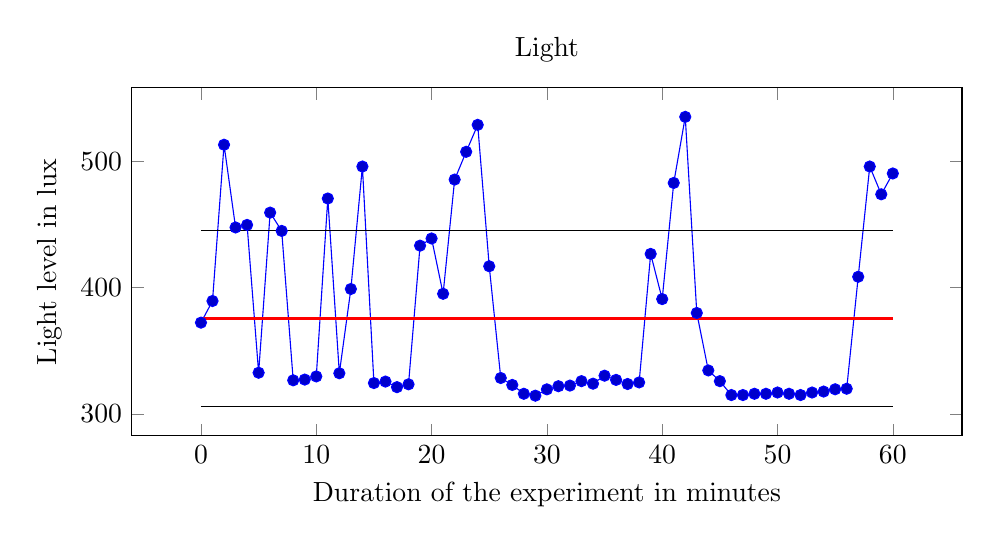
\begin{tikzpicture}
\begin{axis}[
	height=6cm,
	width=\textwidth,
	xlabel=Duration of the experiment in minutes,
	ylabel=Light level in lux,
	title=Light,
	unbounded coords=discard],
	
\addplot coordinates {
(0 , 372.352941176)
(1 , 389.5)
(2 , 513.25)
(3 , 447.75)
(4 , 449.75)
(5 , 332.666666667)
(6 , 459.5)
(7 , 445.0)
(8 , 326.666666667)
(9 , 327.25)
(10 , 329.75)
(11 , 470.666666667)
(12 , 332.25)
(13 , 399.0)
(14 , 496.0)
(15 , 324.5)
(16 , 325.666666667)
(17 , 321.25)
(18 , 323.5)
(19 , 433.333333333)
(20 , 439.0)
(21 , 395.2)
(22 , 485.666666667)
(23 , 507.666666667)
(24 , 529.0)
(25 , 417.0)
(26 , 328.5)
(27 , 323.0)
(28 , 316.0)
(29 , 314.5)
(30 , 319.5)
(31 , 322.0)
(32 , 322.5)
(33 , 326.0)
(34 , 324.0)
(35 , 330.333333333)
(36 , 327.0)
(37 , 323.75)
(38 , 325.0)
(39 , 426.8)
(40 , 391.0)
(41 , 483.0)
(42 , 535.333333333)
(43 , 380.0)
(44 , 334.5)
(45 , 326.0)
(46 , 315.0)
(47 , 315.0)
(48 , 316.0)
(49 , 316.0)
(50 , 317.0)
(51 , 316.0)
(52 , 315.0)
(53 , 317.0)
(54 , 317.75)
(55 , 319.571428571)
(56 , 320.0)
(57 , 408.684210526)
(58 , 496.0)
(59 , 474.0)
(60 , 490.5)
};

\addplot[mark=none, red, very thick] coordinates {(0, 375.580976338) (60, 375.580976338)};

\addplot[mark=none, black] coordinates {(0, 305.697485999) (60, 305.697485999)};
\addplot[mark=none, black] coordinates {(0, 445.464466676) (60, 445.464466676)};


\end{axis}
\end{tikzpicture}
 	\vspace{5 mm}
\end{figure}

\newpage
\FloatBarrier
\newpage
\subsection{Noise Level}
\begin{figure}[ht]
	\centering
	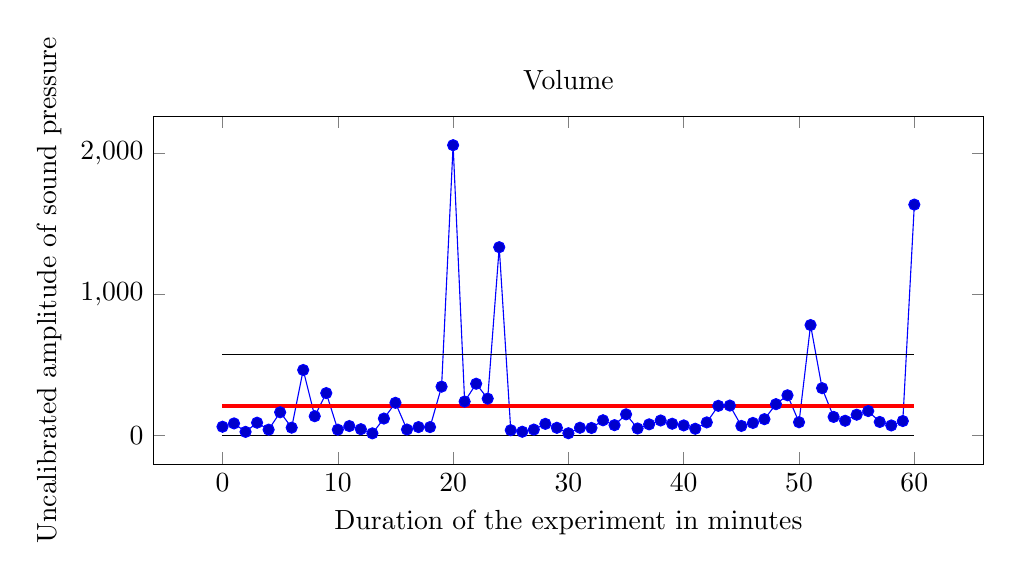
\begin{tikzpicture}
\begin{axis}[
	height=6cm,
	width=\textwidth,
	ylabel=Uncalibrated amplitude of sound pressure,
	xlabel=Duration of the experiment in minutes,
	title=Volume,
	unbounded coords=discard],

\addplot coordinates {
(0 , 59.5882352941)
(1 , 83.125)
(2 , 23.0)
(3 , 88.25)
(4 , 38.75)
(5 , 162.333333333)
(6 , 53.0)
(7 , 462.666666667)
(8 , 134.333333333)
(9 , 298.5)
(10 , 38.5)
(11 , 64.3333333333)
(12 , 42.0)
(13 , 12.5)
(14 , 117.75)
(15 , 229.5)
(16 , 39.6666666667)
(17 , 57.0)
(18 , 57.0)
(19 , 344.333333333)
(20 , 2060.0)
(21 , 238.6)
(22 , 365.0)
(23 , 259.0)
(24 , 1335.16666667)
(25 , 35.0)
(26 , 24.0)
(27 , 39.3333333333)
(28 , 80.0)
(29 , 52.0)
(30 , 13.25)
(31 , 52.3333333333)
(32 , 50.75)
(33 , 105.5)
(34 , 70.75)
(35 , 147.666666667)
(36 , 47.0)
(37 , 76.5)
(38 , 104.0)
(39 , 80.8)
(40 , 69.0)
(41 , 45.1666666667)
(42 , 90.3333333333)
(43 , 208.0)
(44 , 210.0)
(45 , 65.3333333333)
(46 , 86.5)
(47 , 113.25)
(48 , 220.0)
(49 , 283.0)
(50 , 91.5)
(51 , 782.0)
(52 , 333.666666667)
(53 , 129.333333333)
(54 , 102.0)
(55 , 145.0)
(56 , 171.0)
(57 , 93.5789473684)
(58 , 68.75)
(59 , 100.0)
(60 , 1637.83333333)
};

\addplot[mark=none, red, very thick] coordinates {(0, 208.000418295) (60, 208.000418295)};

\addplot[mark=none, black] coordinates {(0, 0) (60, 0)};
\addplot[mark=none, black] coordinates {(0, 571.657643466) (60, 571.657643466)};

\end{axis}
\end{tikzpicture}
 	\vspace{5 mm}
\end{figure}

\FloatBarrier

\subsection{Location}
53.3437734, -6.2510318

Dublin, Ireland 

\FloatBarrier
\clearpage
\section{Participant 5}

%HS

\subsection{Date \& Time}
\begin{table}[ht]
  \begin{tabular}{|P{3cm}|P{3cm}|}
	\multicolumn{2}{c}{\textbf{2016-08-09}}    	\\ \hline
    Start Time      			& End Time   					\\ \hline
   \textbf{15:49:28} 	& \textbf{17:20:58}    	\\ \hline
   \multicolumn{2}{c}{Duration}    						\\ \hline
   \multicolumn{2}{c}{\textbf{01:31:30}} 			\\ \hline
  \end{tabular}
  \newline\newline
  \caption{P5: Date and Time}\label{dandt5}
\end{table}

\FloatBarrier

\subsection{Questions}
\begin{itemize} 
  \item[\Checkmark] Are you a Student?
  \item[\XSolidBrush] Did you work in a team?
  \item[\XSolidBrush] Did you listen to music?
  \item[\XSolidBrush] Did you feel tired?
  \item[\Checkmark] Did you enjoy the tasks?
  \item[\Checkmark] Did you give all you attention to the tasks?
  \item[\XSolidBrush] Were you distracted during the tasks?
  \item[\XSolidBrush] Did you feel stressed
  \item[\XSolidBrush] Do you think the tasks were easy?  
\end{itemize}


\FloatBarrier
\newpage
\subsection{Accelerometer}

\begin{figure}[ht]
	\centering
	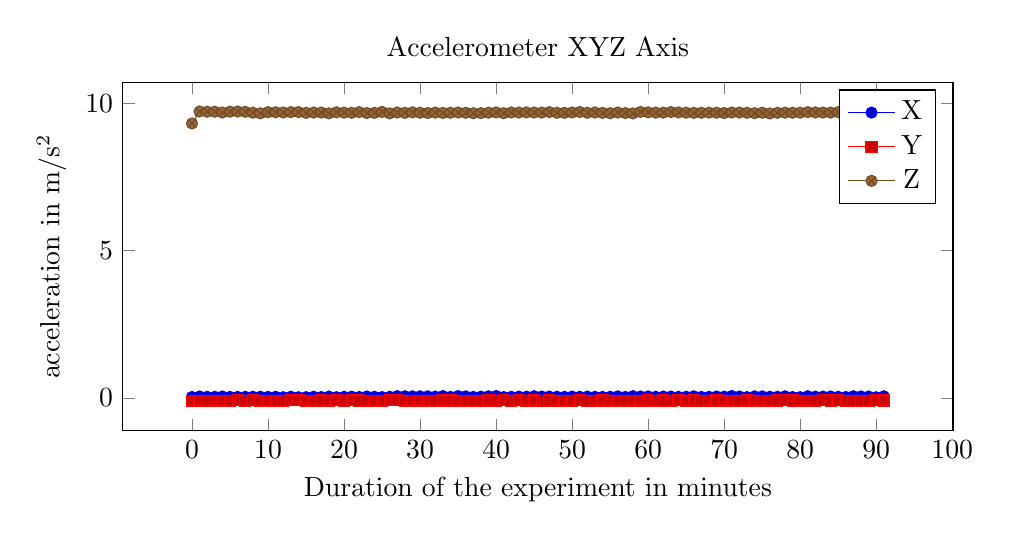
\begin{tikzpicture}
\begin{axis}[
	height=6cm,
	width=\textwidth,
	xlabel=Duration of the experiment in minutes,
	ylabel=acceleration in m/s$^2$,
	title=Accelerometer XYZ Axis,
	unbounded coords=discard],
	
%X
\addplot coordinates {
(0 , 0.028624852325)
(1 , 0.0456503159435)
(2 , 0.0345175602857)
(3 , 0.0348083495)
(4 , 0.04493713425)
(5 , 0.03185272225)
(6 , 0.032054901)
(7 , 0.0333658853333)
(8 , 0.03527832025)
(9 , 0.037109375)
(10 , 0.0322875975)
(11 , 0.036422729)
(12 , 0.02068481454)
(13 , 0.0372229681111)
(14 , 0.0187072753833)
(15 , 0.02278137175)
(16 , 0.0373102818333)
(17 , 0.0263108474615)
(18 , 0.0425605775)
(19 , 0.021026611)
(20 , 0.0350392652833)
(21 , 0.0383300785)
(22 , 0.0275421141)
(23 , 0.0451100666667)
(24 , 0.035198212)
(25 , 0.023899078475)
(26 , 0.035690308)
(27 , 0.05596923825)
(28 , 0.05286331185)
(29 , 0.0494931539167)
(30 , 0.0507286924444)
(31 , 0.0508575438)
(32 , 0.0422706605)
(33 , 0.0589447026667)
(34 , 0.03134918226)
(35 , 0.0602783198)
(36 , 0.0494422905)
(37 , 0.031689962)
(38 , 0.039909362)
(39 , 0.050775147)
(40 , 0.0615295414)
(41 , 0.0245971678667)
(42 , 0.0336181642)
(43 , 0.04070663425)
(44 , 0.038182577)
(45 , 0.05458831725)
(46 , 0.043797811)
(47 , 0.0426910398)
(48 , 0.0372436522)
(49 , 0.0326446532)
(50 , 0.0426849356)
(51 , 0.0350494386667)
(52 , 0.04183197075)
(53 , 0.03400802625)
(54 , 0.030904134)
(55 , 0.034921264)
(56 , 0.049016317)
(57 , 0.0298919676667)
(58 , 0.055935669)
(59 , 0.045284271)
(60 , 0.0474853525)
(61 , 0.0355326333333)
(62 , 0.04415130625)
(63 , 0.04241180425)
(64 , 0.0335184733333)
(65 , 0.0360717774)
(66 , 0.05042648375)
(67 , 0.03061294525)
(68 , 0.0333030008182)
(69 , 0.0442055152105)
(70 , 0.040286255)
(71 , 0.0616607675)
(72 , 0.0454444895)
(73 , 0.024180095)
(74 , 0.049064636)
(75 , 0.0488922114)
(76 , 0.03613281275)
(77 , 0.03391647325)
(78 , 0.0513407386667)
(79 , 0.0258255005)
(80 , 0.023609161425)
(81 , 0.054763794)
(82 , 0.0396626796667)
(83 , 0.04229354875)
(84 , 0.0447021485)
(85 , 0.0336486822)
(86 , 0.0279922485)
(87 , 0.0545578005)
(88 , 0.0470581055)
(89 , 0.0445327755)
(90 , 0.019207001)
(91 , 0.05170059225)
};

%Y
\addplot coordinates {
(0 , -0.09772237125)
(1 , -0.108810424783)
(2 , -0.103489468571)
(3 , -0.105393982)
(4 , -0.1029891965)
(5 , -0.09886169375)
(6 , -0.087383271)
(7 , -0.0943857833333)
(8 , -0.08496475)
(9 , -0.0982716866667)
(10 , -0.09655761625)
(11 , -0.0961120602)
(12 , -0.107305908)
(13 , -0.081837973)
(14 , -0.0802561431667)
(15 , -0.095504761)
(16 , -0.0975189198333)
(17 , -0.0929166354615)
(18 , -0.097572326)
(19 , -0.0717506415)
(20 , -0.0957183841667)
(21 , -0.08687210025)
(22 , -0.09144973825)
(23 , -0.09747823)
(24 , -0.101642611)
(25 , -0.1035652175)
(26 , -0.066518148)
(27 , -0.08568573)
(28 , -0.10135345475)
(29 , -0.102905273208)
(30 , -0.10242886)
(31 , -0.1043487568)
(32 , -0.102169036)
(33 , -0.091405232)
(34 , -0.09143066375)
(35 , -0.1044128416)
(36 , -0.10267639)
(37 , -0.1101964315)
(38 , -0.1020584125)
(39 , -0.0895660396)
(40 , -0.1017395028)
(41 , -0.0832926433333)
(42 , -0.102542115)
(43 , -0.087623596)
(44 , -0.0957692433333)
(45 , -0.09049987875)
(46 , -0.0987981168333)
(47 , -0.090505982)
(48 , -0.0970825196)
(49 , -0.095925903)
(50 , -0.103506469)
(51 , -0.087066651)
(52 , -0.10188675)
(53 , -0.10551452675)
(54 , -0.0904235846667)
(55 , -0.0952545168)
(56 , -0.100504556667)
(57 , -0.105763753333)
(58 , -0.098510743)
(59 , -0.104553225)
(60 , -0.089305879)
(61 , -0.120956418667)
(62 , -0.0916442855)
(63 , -0.105182646)
(64 , -0.082397462)
(65 , -0.101950074)
(66 , -0.09177398725)
(67 , -0.0966796875)
(68 , -0.0961914064545)
(69 , -0.0925381308421)
(70 , -0.1081848152)
(71 , -0.0940208435)
(72 , -0.09459114075)
(73 , -0.0914408366667)
(74 , -0.095474245)
(75 , -0.101541138)
(76 , -0.110935209)
(77 , -0.087963105)
(78 , -0.086324055)
(79 , -0.090545655)
(80 , -0.11132431)
(81 , -0.09964752125)
(82 , -0.12154134)
(83 , -0.07924652)
(84 , -0.0934127799)
(85 , -0.0864471432)
(86 , -0.09584426875)
(87 , -0.099739075)
(88 , -0.1060752875)
(89 , -0.09546661375)
(90 , -0.0802040115)
(91 , -0.0905571)
};

%Z
\addplot coordinates {
(0 , 9.3104775)
(1 , 9.71597156522)
(2 , 9.70799707143)
(3 , 9.7079117)
(4 , 9.68053425)
(5 , 9.71026225)
(6 , 9.715645)
(7 , 9.70654266667)
(8 , 9.675411)
(9 , 9.65371166667)
(10 , 9.693695)
(11 , 9.6893708)
(12 , 9.6818605)
(13 , 9.69282183333)
(14 , 9.69518283333)
(15 , 9.669311625)
(16 , 9.68030308333)
(17 , 9.67978007692)
(18 , 9.65250425)
(19 , 9.68883525)
(20 , 9.67687475)
(21 , 9.6719855)
(22 , 9.695724375)
(23 , 9.66287733333)
(24 , 9.66836925)
(25 , 9.70105)
(26 , 9.651494)
(27 , 9.681896)
(28 , 9.66984335)
(29 , 9.68622652083)
(30 , 9.67309044444)
(31 , 9.6627592)
(32 , 9.6778755)
(33 , 9.66750083333)
(34 , 9.673275)
(35 , 9.6826139)
(36 , 9.671501)
(37 , 9.65692133333)
(38 , 9.661518)
(39 , 9.6754394)
(40 , 9.6855011)
(41 , 9.657328)
(42 , 9.6824404)
(43 , 9.68023675)
(44 , 9.684133)
(45 , 9.68102275)
(46 , 9.67905545833)
(47 , 9.6964352)
(48 , 9.6722078)
(49 , 9.6715148)
(50 , 9.6816741)
(51 , 9.698008)
(52 , 9.6722985)
(53 , 9.682353875)
(54 , 9.669093)
(55 , 9.6570252)
(56 , 9.68032066667)
(57 , 9.66158566667)
(58 , 9.6507874)
(59 , 9.69986325)
(60 , 9.68689325)
(61 , 9.67655433333)
(62 , 9.67766575)
(63 , 9.698765)
(64 , 9.68428016667)
(65 , 9.6757873)
(66 , 9.670021125)
(67 , 9.67202375)
(68 , 9.67732095455)
(69 , 9.67484878947)
(70 , 9.6626556)
(71 , 9.68144225)
(72 , 9.68019875)
(73 , 9.67266333333)
(74 , 9.65867975)
(75 , 9.6737824)
(76 , 9.648448875)
(77 , 9.671032)
(78 , 9.67692066667)
(79 , 9.674061)
(80 , 9.675293)
(81 , 9.6954535)
(82 , 9.68317666667)
(83 , 9.679886)
(84 , 9.677974)
(85 , 9.6936248)
(86 , 9.65489175)
(87 , 9.67543025)
(88 , 9.66282675)
(89 , 9.66626375)
(90 , 9.68290325)
(91 , 9.6799165)
};

\addlegendentry{X}
\addlegendentry{Y}
\addlegendentry{Z}
\end{axis}
\end{tikzpicture}
 	\vspace{5 mm}
\end{figure}

\FloatBarrier
\subsection{Light Level}
\begin{figure}[ht]
	\centering
	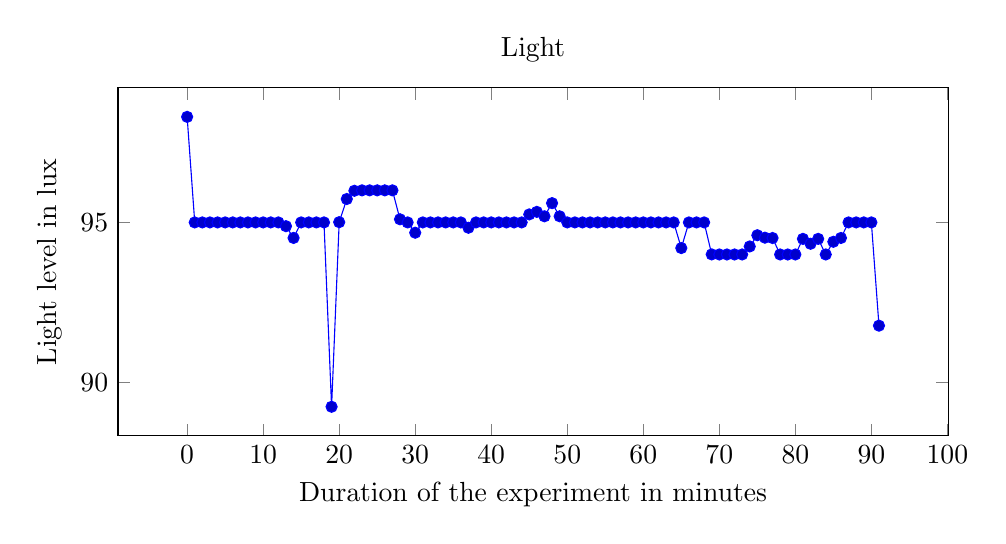
\begin{tikzpicture}
\begin{axis}[
	height=6cm,
	width=\textwidth,
	xlabel=Duration of the experiment in minutes,
	ylabel=Light level in lux,
	title=Light,
	unbounded coords=discard],
	
\addplot coordinates {
(0 , 98.2916666667)
(1 , 95.0)
(2 , 95.0)
(3 , 95.0)
(4 , 95.0)
(5 , 95.0)
(6 , 95.0)
(7 , 95.0)
(8 , 95.0)
(9 , 95.0)
(10 , 95.0)
(11 , 95.0)
(12 , 95.0)
(13 , 94.8825577778)
(14 , 94.5164273333)
(15 , 95.0)
(16 , 95.0)
(17 , 95.0)
(18 , 95.0)
(19 , 89.25)
(20 , 95.0078283333)
(21 , 95.7297625)
(22 , 95.986889)
(23 , 96.0)
(24 , 96.0)
(25 , 96.0)
(26 , 96.0)
(27 , 96.0)
(28 , 95.0976655)
(29 , 95.0)
(30 , 94.678594)
(31 , 95.0)
(32 , 95.0)
(33 , 95.0)
(34 , 95.0)
(35 , 95.0)
(36 , 95.0)
(37 , 94.8333333333)
(38 , 95.0)
(39 , 95.0)
(40 , 95.0)
(41 , 95.0)
(42 , 95.0)
(43 , 95.0)
(44 , 95.0)
(45 , 95.25)
(46 , 95.3285295)
(47 , 95.190542)
(48 , 95.601148)
(49 , 95.190604)
(50 , 95.0)
(51 , 95.0)
(52 , 95.0)
(53 , 95.0)
(54 , 95.0)
(55 , 95.0)
(56 , 95.0)
(57 , 95.0)
(58 , 95.0)
(59 , 95.0)
(60 , 95.0)
(61 , 95.0)
(62 , 95.0)
(63 , 95.0)
(64 , 95.0)
(65 , 94.2)
(66 , 95.0)
(67 , 95.0)
(68 , 95.0)
(69 , 94.0025184211)
(70 , 94.0)
(71 , 94.0)
(72 , 94.0)
(73 , 94.0)
(74 , 94.25)
(75 , 94.6)
(76 , 94.524485)
(77 , 94.5133925)
(78 , 94.0)
(79 , 94.0)
(80 , 94.0)
(81 , 94.48627)
(82 , 94.3333333333)
(83 , 94.486889)
(84 , 94.0)
(85 , 94.3959052)
(86 , 94.5150075)
(87 , 95.0)
(88 , 95.0)
(89 , 95.0)
(90 , 95.0)
(91 , 91.78003)
};

\end{axis}
\end{tikzpicture}
 	\vspace{5 mm}
\end{figure}

\newpage
\FloatBarrier
\newpage
\subsection{Noise Level}
\begin{figure}[ht]
	\centering
	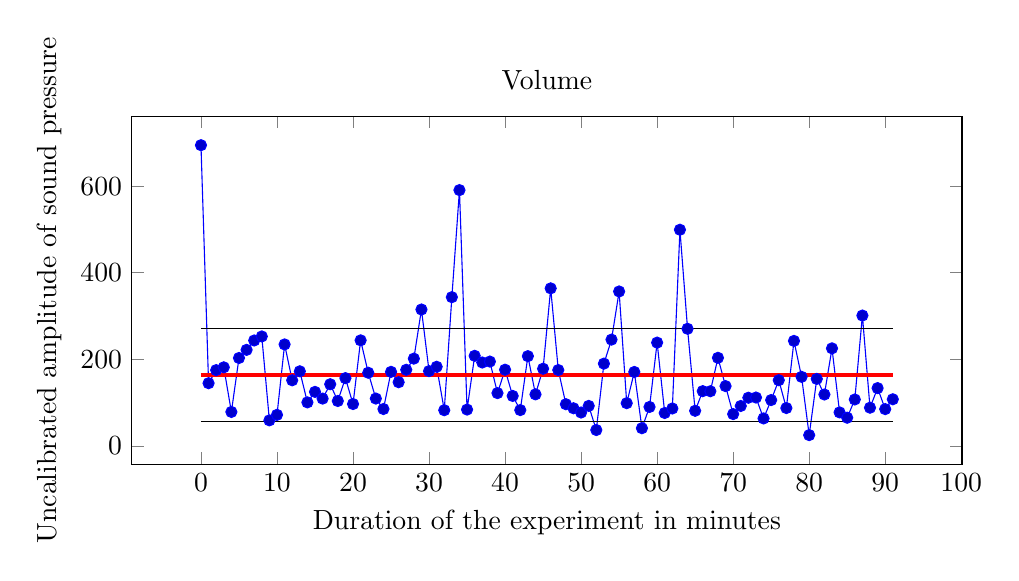
\begin{tikzpicture}
\begin{axis}[
	height=6cm,
	width=\textwidth,
	ylabel=Uncalibrated amplitude of sound pressure,
	xlabel=Duration of the experiment in minutes,
	title=Volume,
	unbounded coords=discard],

\addplot coordinates {
(0 , 694.416666667)
(1 , 145.086956522)
(2 , 175.285714286)
(3 , 181.7)
(4 , 78.75)
(5 , 203.25)
(6 , 222.0)
(7 , 243.666666667)
(8 , 253.0)
(9 , 59.3333333333)
(10 , 72.0)
(11 , 234.6)
(12 , 151.8)
(13 , 172.555555556)
(14 , 100.833333333)
(15 , 125.0)
(16 , 109.5)
(17 , 142.692307692)
(18 , 104.0)
(19 , 156.75)
(20 , 97.0)
(21 , 244.0)
(22 , 169.25)
(23 , 109.666666667)
(24 , 85.5)
(25 , 171.25)
(26 , 147.333333333)
(27 , 176.0)
(28 , 201.8)
(29 , 315.166666667)
(30 , 173.0)
(31 , 183.0)
(32 , 82.75)
(33 , 343.666666667)
(34 , 590.75)
(35 , 84.2)
(36 , 208.25)
(37 , 192.833333333)
(38 , 195.0)
(39 , 122.2)
(40 , 176.2)
(41 , 115.666666667)
(42 , 83.0)
(43 , 207.5)
(44 , 119.333333333)
(45 , 178.5)
(46 , 364.0)
(47 , 175.4)
(48 , 96.6)
(49 , 87.2)
(50 , 77.4)
(51 , 92.6666666667)
(52 , 37.0)
(53 , 190.25)
(54 , 245.666666667)
(55 , 356.8)
(56 , 99.0)
(57 , 171.0)
(58 , 41.2)
(59 , 90.25)
(60 , 238.75)
(61 , 76.3333333333)
(62 , 86.75)
(63 , 499.25)
(64 , 270.666666667)
(65 , 81.4)
(66 , 126.75)
(67 , 126.5)
(68 , 203.636363636)
(69 , 138.368421053)
(70 , 73.8)
(71 , 92.5)
(72 , 111.5)
(73 , 112.0)
(74 , 63.75)
(75 , 106.2)
(76 , 152.0)
(77 , 87.75)
(78 , 242.666666667)
(79 , 159.75)
(80 , 25.25)
(81 , 155.0)
(82 , 119.0)
(83 , 225.5)
(84 , 77.7)
(85 , 65.4)
(86 , 107.5)
(87 , 301.25)
(88 , 88.5)
(89 , 133.75)
(90 , 85.25)
(91 , 108.0)
};

\addplot[mark=none, red, very thick] coordinates {(0, 163.759695494) (91, 163.759695494)};

\addplot[mark=none, black] coordinates {(0, 56.1651969983) (91, 56.1651969983)};
\addplot[mark=none, black] coordinates {(0, 271.354193989) (91, 271.354193989)};

\end{axis}
\end{tikzpicture}
 	\vspace{5 mm}
\end{figure}

\FloatBarrier

\subsection{Location}
-6.250537, 53.3437789

Dublin, Ireland

\FloatBarrier